% !TeX root = thesis.tex
\chapter{Introduction}\label{C:intro}

% =====================================================================
\section{Motivation}\label{S:intro:motivation}
% =====================================================================

A time series is a collection of observations $\{x_t\}$, each regarded as a realised value of a random variable $X_t$, indexed by discrete or continuous time.
Time series carry information about the system that generates them, and their analysis is central to engineering, economics and the physical, biological and Earth sciences.
Typical applications include the analysis of exchange rates and commodity prices in finance, the growth and decline of bacterial populations in biology, the spread of diseases such as COVID-19 or influenza in medicine, and the prediction of wet and dry days in geoscience (Figure~\ref{fig:timeseries}).

\begin{figure}[hbt]
	\centering
	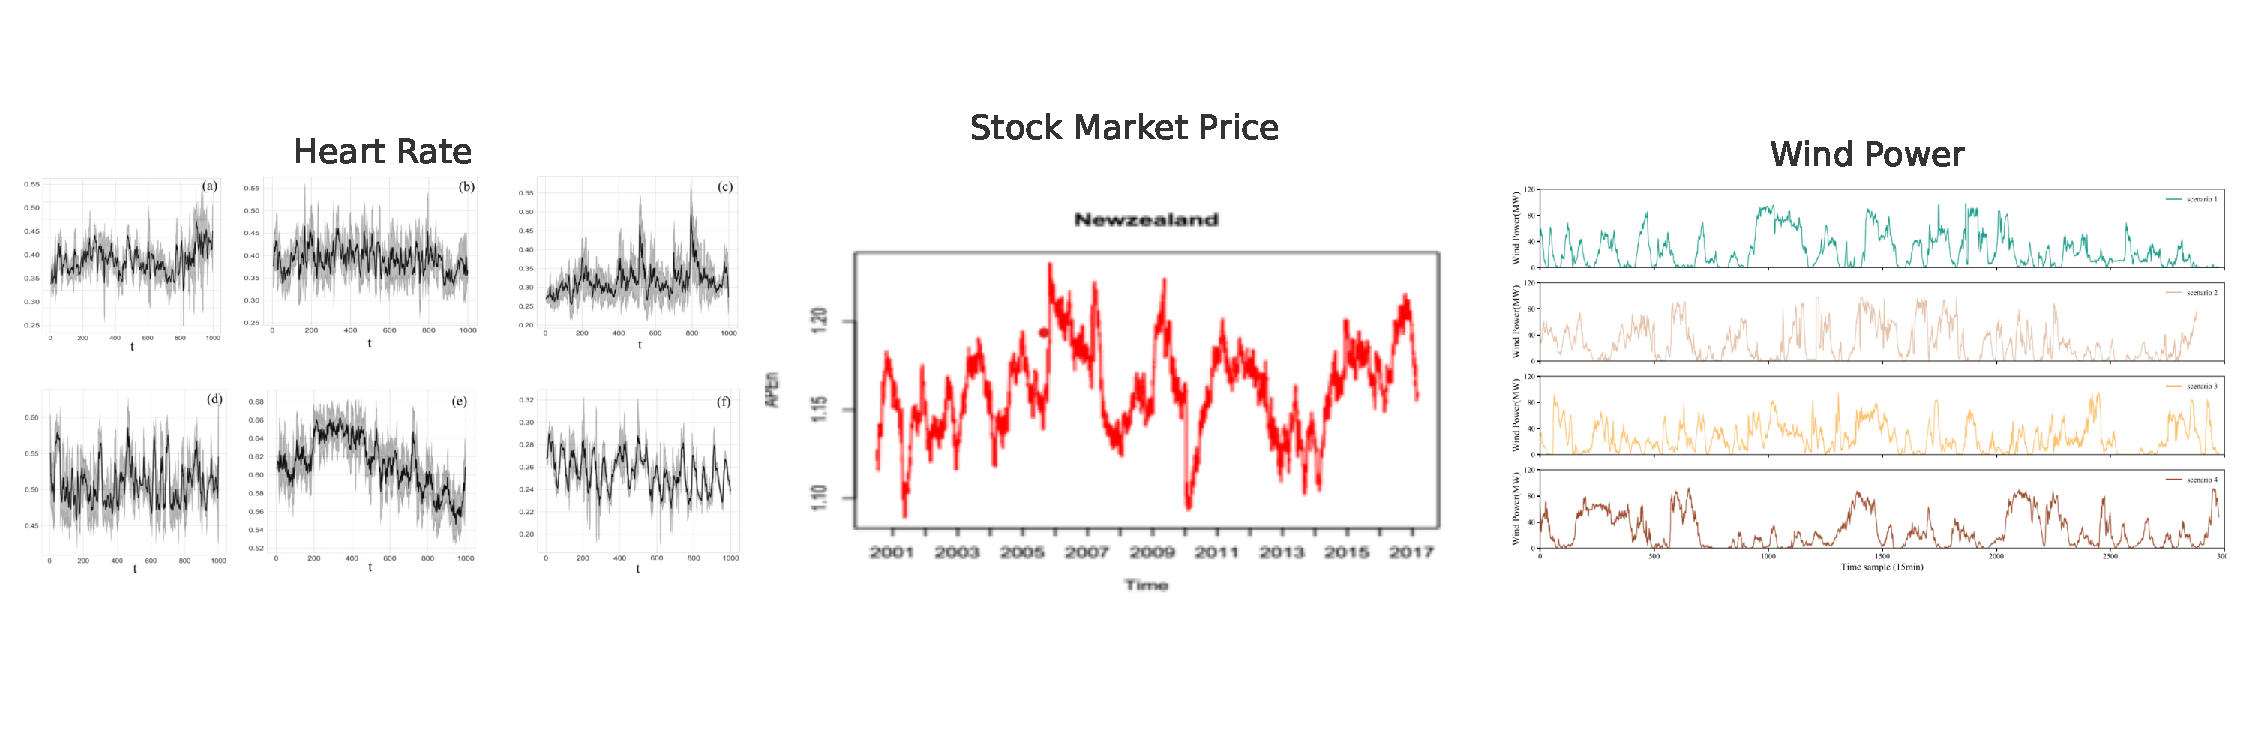
\includegraphics[width=0.99\textwidth]{Figures/Chapter1/time series plots}
	\caption{Examples of time series from biology, finance and geoscience. Sources: Silva et al., Patra et al.\ and Meng et al.~\cite{Silva2023,Patra2022,Meng2023}.}
	\label{fig:timeseries}
\end{figure}

The two classical families of methods are time-domain and frequency-domain analysis.
Time-domain methods, based on autocorrelation and regression, relate the present value of a series to its own past or to the past of other series.
Frequency-domain methods represent a series through spectral expansions such as Fourier modes or wavelets~\cite{treitel1995spectral}.
Both families typically rely on assumptions such as linearity, stationarity, Gaussianity or large sample sizes.
Real-world data frequently violate these assumptions: geophysical and remote-sensing records, for instance, are noisy, non-stationary, contain outliers and are often short relative to the phenomena of interest.
When the assumptions fail, the resulting inferences can be biased or misleading.

Classical non-parametric statistics address part of this problem by working with the ranks of the observations instead of their values, but most rank-based procedures ignore the temporal ordering that makes a time series informative.
Ordinal-pattern analysis, introduced by Bandt and Pompe~\cite{PhysRevLett.88.174102}, combines both ideas: it uses only the relative order of observations, and it does so locally, along the time axis.

% =====================================================================
\section{Ordinal patterns}\label{S:intro:op}
% =====================================================================

The Bandt and Pompe method transforms short, consecutive segments of a time series into symbols that encode the order relations among their values.
The empirical distribution of these symbols is then summarised by information-theoretic descriptors.
Because only order relations are used, the resulting distribution does not depend on any parametric model, is invariant to monotonic transformations of the data, and is robust to outliers and to observational noise.
The method is also computationally inexpensive.
Since 2002 it has been applied in biomedical signal processing, optical chaos, hydrology, geophysics, econophysics, engineering and biometrics, and to the assessment of pseudo-random number generators~\cite{Zanin2012}.

Formally, let $\bm{x}=(x_1,x_2,\dots,x_{n+D-1})$ be a real-valued time series of length $n+D-1$ without ties.
For an embedding dimension $D$ (usually $3\le D\le 6$) and unit time delay, each window $(x_j,\dots,x_{j+D-1})$, $1\le j\le n$, is mapped to one of the $D!$ possible permutations of $\{1,\dots,D\}$.
In this thesis each window is encoded by the vector of ranks of its values.
This yields the symbol sequence $\bm{\pi}=(\pi_1,\dots,\pi_n)$ with $\pi_j\in\{\pi^1,\dots,\pi^{D!}\}$, and the histogram of proportions $\bm{h}=(h_1,\dots,h_{k})$, $k=D!$, where $h_\ell$ is the proportion of symbols of type $\pi^\ell$.
For statistical purposes we model the symbol counts as a $k$-dimensional multinomial random vector.

% ---------------------------------------------------------------------
\subsection{An illustrative example}\label{S:intro:example}
% ---------------------------------------------------------------------

Consider the mean monthly relative humidity in Wellington (Table~\ref{tab:humidity} and Figure~\ref{fig:humidity}).

\begin{table}[hbt]
	\centering
	\begin{tabular}{lc}
		\toprule
		Month & Mean relative humidity (\%) \\
		\midrule
		January & 77.3 \\
		February & 81.0 \\
		March & 82.4 \\
		April & 81.7 \\
		May & 83.6 \\
		June & 85.6 \\
		July & 84.4 \\
		August & 83.1 \\
		September & 78.8 \\
		October & 79.6 \\
		November & 78.2 \\
		December & 78.8 \\
		\bottomrule
	\end{tabular}
	\caption{Mean monthly relative humidity in Wellington.}
	\label{tab:humidity}
\end{table}

\begin{figure}[hbt]
	\centering
	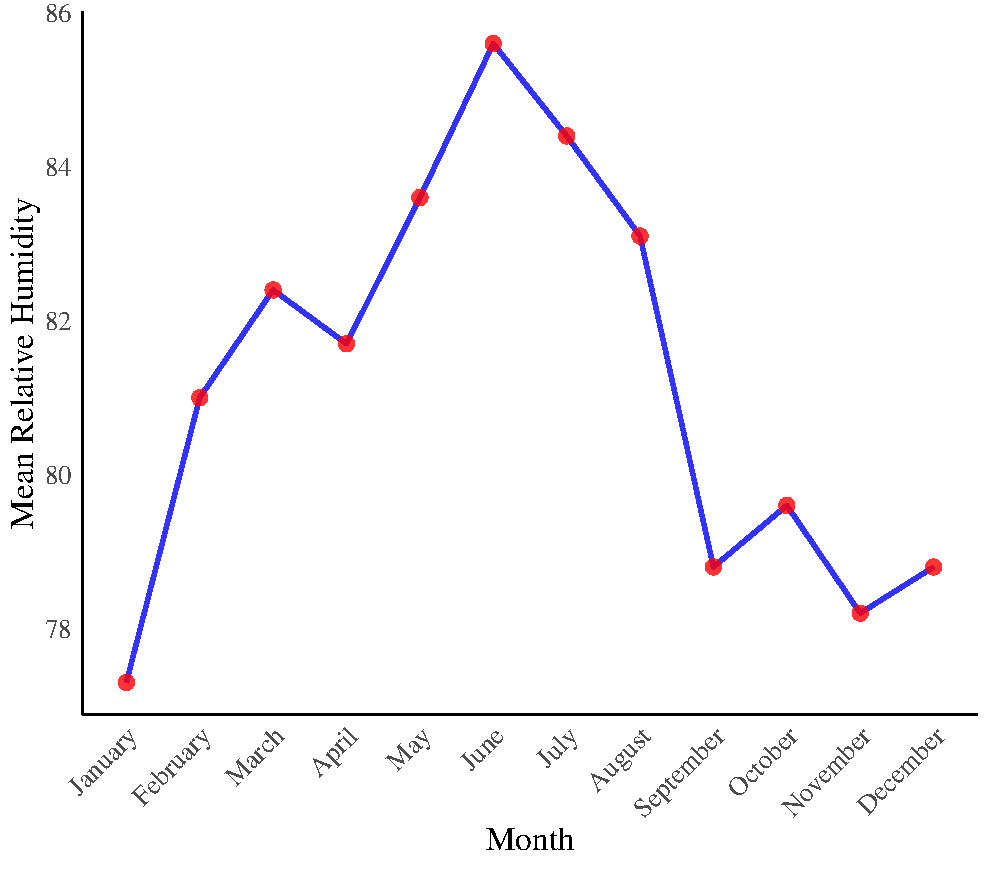
\includegraphics[width=0.6\textwidth]{Figures/Chapter1/humidity graph}
	\caption{Mean monthly relative humidity in Wellington.}
	\label{fig:humidity}
\end{figure}

With $D=3$, the first overlapping window $(77.3, 81.0, 82.4)$ is increasing: $77.3$ receives rank $1$, $81.0$ rank $2$ and $82.4$ rank $3$, giving the pattern $(123)$.
The window $(83.1, 78.8, 79.6)$ gives the pattern $(312)$, since $83.1$ is the largest value, $78.8$ the smallest and $79.6$ the intermediate one.
Proceeding in this way, the $12$ observations produce $n=10$ patterns (Table~\ref{tab:op}).

\begin{table}[hbt]
	\centering
	\begin{tabular}{lcr}
		\toprule
		$t$ & Window & Ordinal pattern \\
		\midrule
		1 & (77.3, 81.0, 82.4) & (123) $=\pi^1$\\
		2 & (81.0, 82.4, 81.7) & (132) $=\pi^2$\\
		3 & (82.4, 81.7, 83.6) & (213) $=\pi^3$\\
		4 & (81.7, 83.6, 85.6) & (123) $=\pi^1$\\
		5 & (83.6, 85.6, 84.4) & (132) $=\pi^2$\\
		6 & (85.6, 84.4, 83.1) & (321) $=\pi^6$\\
		7 & (84.4, 83.1, 78.8) & (321) $=\pi^6$\\
		8 & (83.1, 78.8, 79.6) & (312) $=\pi^5$\\
		9 & (78.8, 79.6, 78.2) & (231) $=\pi^4$\\
		10 & (79.6, 78.2, 78.8) & (312) $=\pi^5$\\
		\bottomrule
	\end{tabular}
	\caption{Ordinal patterns of dimension $D=3$ for the series in Table~\ref{tab:humidity}.}
	\label{tab:op}
\end{table}

The six possible patterns are $\{\pi^1,\dots,\pi^6\}=\{(123),(132),(213),(231),(312),(321)\}$, and their relative frequencies are
\begin{equation}
	\hat{p}_i=\frac{\#\{\pi_j\in\bm{\pi}:\pi_j=\pi^i\}}{n},\qquad 1\le i\le 6,
\end{equation}
giving $\hat{\bm{p}}=(2,2,1,1,2,2)/10$ (Table~\ref{tab:probability_function} and Figure~\ref{fig:histogram}).

\begin{table}[hbt]
	\centering
	\begin{tabular}{lc}
		\toprule
		Pattern & Relative frequency \\
		\midrule
		$\pi^1$ & $2/10$ \\
		$\pi^2$ & $2/10$ \\
		$\pi^3$ & $1/10$ \\
		$\pi^4$ & $1/10$ \\
		$\pi^5$ & $2/10$ \\
		$\pi^6$ & $2/10$ \\
		\bottomrule
	\end{tabular}
	\caption{Empirical distribution of ordinal patterns for the humidity series.}
	\label{tab:probability_function}
\end{table}

\begin{figure}[hbt]
	\centering
	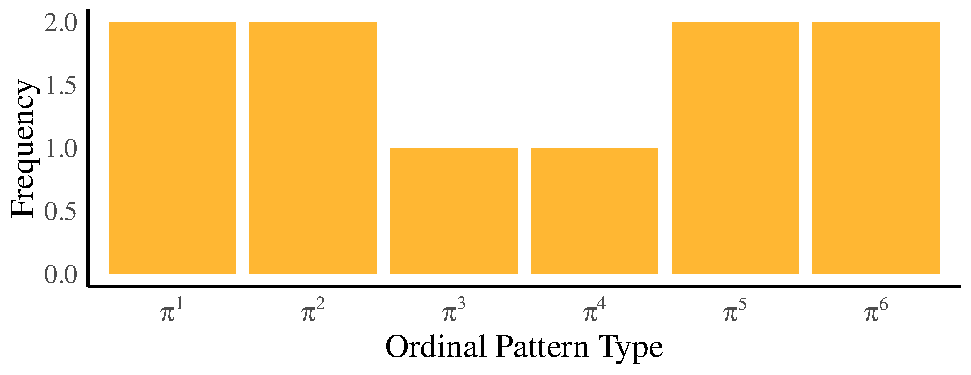
\includegraphics[width=0.6\textwidth]{Figures/Chapter1/frequency histogram}
	\caption{Histogram of the proportions of observed patterns (Table~\ref{tab:probability_function}).}
	\label{fig:histogram}
\end{figure}

All the features studied in this thesis are functions of distributions such as $\hat{\bm p}$.
In practice, much longer series are needed: with $D$ patterns there are $D!$ bins to estimate, and reliable estimation requires $n\gg D!$.

% =====================================================================
\section{From ordinal patterns to features}\label{S:intro:features}
% =====================================================================

Bandt and Pompe summarised $\hat{\bm p}$ by its normalised Shannon entropy, known as permutation entropy~\cite{PhysRevLett.88.174102}.
Entropy alone, however, does not distinguish all types of dynamics.
L\'opez-Ruiz et al.~\cite{lopez1995statistical} introduced statistical complexity as the product of entropy and a disequilibrium term measuring the distance to the uniform distribution.
Lamberti et al.~\cite{lamberti2004intensive} replaced the Euclidean distance with the Jensen--Shannon divergence, which gives an intensive measure.
Rosso et al.~\cite{Rosso2007} proposed representing each series as a point in the entropy--complexity ($H\times C$) plane, and Martin et al.~\cite{Martin2006} derived the curves that bound the attainable region of this plane.
Generalised entropies (R\'enyi and Tsallis) and the Fisher information measure, which is sensitive to local changes in the distribution, provide further descriptors.
Because all these features are estimated from finite samples, their sampling variability matters.
Rey et al.~\cite{Rey2024} derived the asymptotic distributions of the Shannon, R\'enyi and Tsallis entropies and of the Fisher information measure of ordinal patterns, which yield variances and confidence intervals for these quantities.

% =====================================================================
\section{Research gap and objectives}\label{S:intro:gap}
% =====================================================================

Ordinal-pattern descriptors are widely used to characterise individual time series, usually one or two at a time, and most often through permutation entropy alone.
Clustering based on ordinal-pattern distributions has been proposed~\cite{Brandmaier2015}.
However, the joint use of a rich set of ordinal-pattern features as a feature space for clustering and classification has received little systematic attention.
Such a feature space would combine several entropies, their complexities, the Fisher information and variance-based measures of stability.
In particular, it is not known:
\begin{itemize}
	\item how these features behave for processes that mix deterministic and stochastic dynamics, which occupy regions of the $H\times C$ plane that pure models do not reach;
	\item which features carry complementary information and which are redundant;
	\item how large a series must be for clustering in this feature space to recover the generating mechanisms;
	\item how well the features perform on real, noisy data from the Earth sciences.
\end{itemize}

The objectives of this thesis are therefore to:
\begin{enumerate}
	\item define a feature space of thirteen ordinal-pattern descriptors, comprising entropies, statistical complexities, the Fisher information measure, the disequilibrium and variance-based stability measures;
	\item study the behaviour of these features through a simulation design based on convex combinations of deterministic and stochastic processes, and assess their ability to support unsupervised clustering of time series;
	\item apply the features to land use/land cover classification of Synthetic Aperture Radar (SAR) time series;
	\item apply the features to the detection of unusual seismic-amplitude behaviour at Whakaari, New Zealand, and assess their relationship with Volcanic Alert Levels and eruptions.
	% \item [Optional, if completed] use event coincidence analysis to quantify the temporal association between feature anomalies and volcanic events.
\end{enumerate}

% =====================================================================
\section{Contributions}\label{S:intro:contrib}
% =====================================================================

The main contributions of this thesis are:
\begin{enumerate}
	\item \textbf{A simulation framework based on convex combinations.} Series of the form $X_t(w)=wX_t^{(S)}+(1-w)X_t^{(D)}$, $0\le w\le 1$, with stochastic components AR(2), MA(2) and ARMA(2,2) and deterministic components the logistic map and a sine function, trace continuous paths in the $H\times C$ plane. These paths populate regions that pure models leave empty.
	\item \textbf{Clustering in an ordinal-pattern feature space.} Fifteen model classes are clustered with $k$-means using the thirteen features. With $n=10\,000$ and $D=4$, the eleven clusters selected by silhouette analysis largely correspond to the generating mechanisms, while only borderline mixtures are split between neighbouring clusters. Clustering degrades markedly for $n=1000$.
	\item \textbf{An assessment of feature redundancy.} The Shannon, R\'enyi and Tsallis entropies are almost perfectly correlated, whereas the Fisher-based and variance-based features carry largely independent information.
	\item \textbf{An application to SAR land cover classification.} Ordinal-pattern features combined with a support vector machine separate Agriculture and Forest well, while Urban and Water remain difficult to distinguish.
	\item \textbf{An application to volcano monitoring.} At Whakaari, unsupervised clustering of weekly RSAM feature windows does not recover the Volcanic Alert Level classes, and supervised classification recovers only some eruption windows. The analysis quantifies both the potential and the current limits of ordinal-pattern features for detecting volcanic unrest.
\end{enumerate}

Parts of this work have been presented in the following publication:
\begin{itemize}
	\item R.~Dilhani, A.~Sabir, U.~Khati, A.~C.~Frery and A.~A.~Rey, ``Land cover classification in SAR time series using ordinal pattern features,'' [venue, year].
\end{itemize}

% =====================================================================
\section{Thesis outline}\label{S:intro:outline}
% =====================================================================

The remainder of this thesis is organised as follows.
Chapter~\ref{C:lit} reviews the literature on ordinal-pattern analysis, information-theoretic quantifiers and their applications to time series clustering and to geophysical and remote-sensing data.
Chapter~\ref{C:features} defines the thirteen ordinal-pattern features, including the Shannon, R\'enyi and Tsallis entropies, the Fisher information measure, the associated statistical complexities and the asymptotic variances used to quantify their stability.
Chapter~\ref{C:sim} presents the convex-combination simulation study and the clustering of simulated time series in the ordinal-pattern feature space.
Chapter~\ref{C:sar} applies the features to land use/land cover classification of SAR time series.
Chapter~\ref{C:seismic} analyses RSAM seismic-amplitude records from Whakaari.
% Chapter~\ref{C:eca} applies event coincidence analysis to ... [optional]
Chapter~\ref{C:concl} summarises the findings, discusses limitations and outlines directions for future research.